\section{Verarbeitung von Anfragen}
\label{chap:query_processing}

Die Verarbeitung von Anfragen\footnote{Auch Query Processing} wird im Allgemeinen durch drei Komponenten realisiert~\cite{croft.chap2}.
Auch die im Rahmen dieser Arbeit erstellte Suchmaschine bildet davon keine Ausnahme.
Dementsprechend werden in den folgenden Abschnitten die Bestandteile User Interaction, Ranking und Evaluation vorgestellt.

\subsection{User Interaction~\cite{croft.chap2}}
\label{chap:user_interaction}

Die Komponente zur Nutzerinteraktion bietet eine Schnittstelle\footnote{Der Quellcode ist in dem Modul
\href{https://github.com/mam10eks/search-homepage-of-university-leipzig/tree/master/search-engine-backend}{search-engine-backend}
enthalten.}
zwischen dem Benutzer und der Suchmaschine.
Um diesem Nutzer eine gewohnte Usability inklusive intuitiver Bedienung zu ermöglichen,
wurden die in der Praxis verbreiteten Standards eingehalten.

\begin{wrapfigure}{H}{0.49\linewidth}
	\vspace*{-0.4cm}
	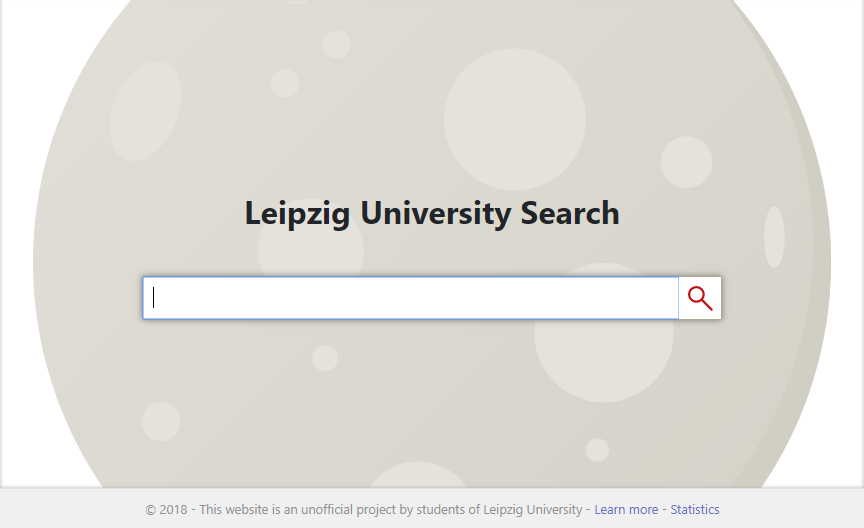
\includegraphics[width=0.48\textwidth]{chapter_query_processing/frontend_landing_page.png}
	\caption{Die Landing Page der Suchmaschine}
	\label{fig:landing_page}
	\vspace*{-0.2cm}
\end{wrapfigure}


Dementsprechend muss einem Nutzer das Absenden von Anfragen ermöglicht werden.
Dafür ist es üblich, eine Landing Page mit prominent mittig platzierter Eingabemaske auszuliefern\cite{baeza_yates.search_interfaces}.
Abbildung~\ref{fig:landing_page} zeigt dies für die im Rahmen dieser Arbeit entwickelte Suchmaschine.

Nachdem ein Nutzer seine Anfrage spezifiziert hat, werden ihm die Ergebnisse präsentiert.
Dafür erhält die Schnittstelle eine für die Query gerankte Liste von Dokumenten von der Ranking-Komponente.
Diesbezüglich ist es gängig, einem Benutzer für kleinere Ausschnitte aus der Dokumentliste jeweils 
ausgewählte Metadaten in Verbindung mit einem 
für die Anfrage besonders relevanten Textausschnitt\footnote{Sogenannte Snippets} zu präsentieren~\cite{baeza_yates.search_interfaces}.
Relevante Wörter werden dabei speziell hervorgehoben.
Die unter Berücksichtigung dieser Punkte entstandene Search Engine Result Page\footnote{SERP} wird in Abbildung~\ref{fig:serp} vorgestellt.

\begin{figure}[!ht]
	
\includegraphics[width=0.99\textwidth]{chapter_query_processing/serp.png}
	\caption{Die SERP für die Anfrage \glqq studiengebühren\grqq}
	\label{fig:serp}
\end{figure}

In der Regel wird einem Nutzer die Formulierung und Spezialisierung seiner Anfragen durch verschiedene Hilfsmittel
erleichtert.
In dem vorliegenden Projekt wurde eine Query Suggestion implementiert,
welche Vervollständigungsvorschläge auf Basis populärer Anfragen liefert.
Die dafür notwendige, dynamische Benutzerschnittstelle wird in Abbildung~\ref{fig:query_suggestions} gezeigt.
Verwandte Maßnahmen zur Verbesserungen der Benutzbarkeit wie Spell Checking oder Query Refinement 
wurden zugunsten anderer Features nicht umgesetzt.

\begin{figure}[!ht]
	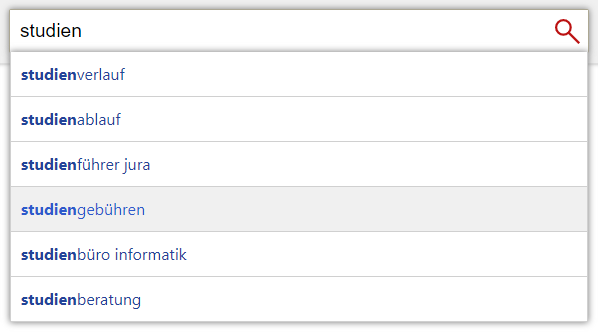
\includegraphics[width=0.99\textwidth]{chapter_query_processing/autocomplete.png}
	\caption{Query Suggestions für die Eingabe: \glqq studien\grqq}
	\label{fig:query_suggestions}
\end{figure}

Um den Suchmaschinenservice einem möglichst breiten Nutzerkreis zuzuführen, sind die
Komponenten zur Benutzerinteraktion in Form eines Webfrontends realisiert. Für die Entwicklung
werden die jeweils aktuellen Standards HTML5, CSS3 sowie JavaScript eingesetzt. 
Ausgeliefert werden diese Bestandteile durch einen Express-Webserver, welcher im Rahmen einer NodeJS-Anwendung betrieben wird.
Aus Kompatibilitätsgründen werden Teile der Bootstrap-Library eingebunden.
Falls ein Browser die History-API unterstützt, wird diese zur
Bereitstellung von Deep-Links ohne einen Full-Page-Refresh
geeigneter Seiten\footnote{Zum Beispiel die About-Page.} verwendet.

Der Zugriff auf die Ranking-Komponente (siehe Abschnitt~\ref{chap:ranking}) und Query-Suggestions wird durch
entsprechende \href{https://en.wikipedia.org/wiki/Representational_state_transfer}{REST-Endpunkte} ermöglicht.
Bereitgestellt werden diese durch eine \href{https://projects.spring.io/spring-boot/}{Spring-Boot-Anwendung}.
Die Query-Suggestions unterscheiden dabei zwischen nutzerbezogenen und globalen Vorschlägen.
Durch nutzerbezogene Vorschläge ist es einem Nutzer möglich, von ihm bereits getätigte Anfragen zu wiederholen.
Globale Vorschläge identifizieren innerhalb der Suchmaschine populäre Anfragen mit Hilfe von Logdaten.
Für eine sinnvolle initiale Menge von globalen Vorschlägen wurden semantisch passende
Vorschläge von Google gecrawlt und eingepflegt\footnote{Der Quellcode für den Crawler ist in dem Modul
\href{https://github.com/mam10eks/search-homepage-of-university-leipzig/tree/master/initial_suggestion_crawling}
{initial\_suggestion\_crawling}.
Damit wurden 2639 Vorschläge generiert}.


\subsection{Ranking~\cite{croft.chap2}}
\label{chap:ranking}
Die Ranking-Komponente ist der Kern jeder Suchmaschine.
Sie erzeugt für eine Query aus der User-Interaction-Komponente eine gerankte Liste von Dokumenten.

Dabei beeinflussen deren Effizienz\footnote{Die Verarbeitung vieler Anfragen in kurzer Zeit.}
und Effektivität\footnote{Die Qualität des Rankings: Kann die Suchmaschine relevante Informationen finden?}
die Nützlichkeit der Suchmaschine wesentlich.
Um für beide Anforderungen einen sinnvollen Ausgangspunkt zu schaffen, wurde für das Ranking
\href{https://lucene.apache.org/}{Lucene} verwendet.
Diese Software stellt einen geeigneten Einstieg dar, da darauf andere,
in dieser Domäne verbreitete Softwarekomponenten aufbauen\footnote{Insbesondere die verbreiteten Tools~\cite{dbengines}
\href{https://de.wikipedia.org/wiki/Elasticsearch}{Elasticsearch} und \href{http://lucene.apache.org/solr/}{Solr}
basieren auf Lucene. Deren erweiterter Funktionsumfang, wie Beispielsweiße eine
\href{http://www.searchdatacenter.de/definition/Horizontale-Skalierung-Scale-out}{horizontale Skalierung}, wurde im Rahmen dieser Arbeit nicht benötigt.}.
Verschiedene \href{https://en.wikipedia.org/wiki/Ranking_(information_retrieval)}{Ranking-Algorithmen}
\footnote{Und damit auch 
\href{https://de.wikipedia.org/wiki/Information_Retrieval\#Retrievalmodelle}{Retrieval-Modelle}}
sind in Lucene verfügbar.

Davon wurde \href{https://en.wikipedia.org/wiki/Okapi_BM25}{BM25F} eingesetzt,
da es als Baseline für modernere Ranking-Algorithmen fungiert und für allgemeine
Dokumentsammlungen bessere Ergebnisse\footnote{Entsprechendes Tuning der von BM25F verwendeten Parameter vorrausgesetzt~\cite{baeza_yates.107}.}
erzielt als die verfügbaren,
\href{https://opensourceconnections.com/blog/2015/10/16/bm25-the-next-generation-of-lucene-relevation/}{klassischen Vektor-Modelle}~\cite{baeza_yates.107}.
Dieses \href{https://de.wikipedia.org/wiki/Information_Retrieval#Retrievalmodelle}{Retrieval-Modell}
besitzt die Fähigkeit, mehrere Felder\footnote{Felder werden auch als Attribute oder Features bezeichnet.} in die Berechnung des Scores einfließen zu lassen.
Entsprechend wurden alle verfügbaren Felder 
einbezogen\footnote{Alle Felder mit unmittelbarem Bezug zu dem Inhalt der Dokumente.
Dies sind der vollständige Text eines Dokuments, sowie deren Titel, URL und Anchor-Texte eingehender Links.}.
Da eine sinnvolle Wahl der Attribute\footnote{Einschließlich eventuell abgeleiteter Features.}
und deren Gewichtung im Allgemeinen in
Verbindung mit der User-Relevanz steht, wurden alle Parameter bei ihren Standards belassen.

Das entsprechende Vorgehen für ein Tuning basierend auf Nutzer-Feedback
wird in Abschnitt~\ref{chap:log_analysis} vorgestellt.



\subsection{Evaluation~\cite{croft.chap2}}
\label{chap:evaluation}
Die Aufgabe der Evaluationskomponente ist es, Effizienz und Effektivität zu monitoren.
Dafür muss eine Aufzeichnung des Nutzerverhaltens sowie ausgewählter Systemmetriken vorgenommen werden.

Insbesondere zur Aufzeichnung des Nutzerverhaltens ist eine Identifikation der Nutzer notwendig.
Darauf aufbauend kann protokolliert werden, welcher Nutzer welche Anfragen ausgeführt
hat, welche Ergebnisseiten oder Query-Suggestions einem Nutzer präsentiert wurden,
sowie gegebenenfalls welche Ergebnisse oder Query Suggestions ausgewählt
wurden\footnote{Das erweitern dieser Informationen um die entsprechenden Event-Zeitpunkte erlaubt eine
sinnvolle Rekonstruktion des Nutzerverhaltens.}.

Bei einer technischen Realisierung dieser Punkte fällt auf,
dass es sich um sogenannte \href{https://de.wikipedia.org/wiki/Cross-Cutting_Concern}{Cross-Cutting Concerns}
handelt. Ein bewährtes Mittel derartige Funktionalitäten zu realisieren, ohne die
Komplexität der betroffenen Systemteile unnötig zu ehöhen,
stellt die Aspektorientierte Programmierung\footnote{AOP} dar\cite{spring.chap1.1}.
Die darin verwendeten Aspekte definieren,
was\footnote{In der zugehörigen AOP Terminologie definiert der zu einem Aspekt gehörende Advice die Aufgabe,
also was von dem Aspekt zu erledigen ist~\cite{spring.chap4.1}.}, wann\footnote{Der Advice eines Aspekts definiert 
neben dem was auch zu welchen Zeitpunkten ein Aspekt auszuführen ist.
Unter anderem kann vor, nach, oder das wrappen einer Zielmethode spezifiziert werden\cite{spring.chap4.1}.}
und wo\footnote{Durch sogenannte Pointcuts werden eine oder mehrere Methoden definiert,
an die der Advice gewoben wird\cite{spring.chap4.1}.} auszuführen ist\cite{spring.chap4.1}.

In dem für die Interaction-Komponente verwendeten Framework werden alle Endpunkte über speziell anotierte Methoden
bereitgestellt.
Diesen ist gemein, dass sie ein
\href{https://de.wikipedia.org/wiki/Plain_Old_Java_Object}{POJO}\footnote{Diese sind 
entsprechend einer gewählten Konvention in dem 
\href{https://github.com/mam10eks/search-homepage-of-university-leipzig/tree/master/search-engine-backend}{Backend-Modul}
in zugehörigen \href{https://de.wikipedia.org/wiki/Transferobjekt}{dto} Paketen definiert.}
als Model für die Antwort zurückgeben. 
Dieses Modell wird je nach Endpunkt später in ein HTML-Template\footnote{Spezifiziert innerhalb des 
\href{https://github.com/mam10eks/search-homepage-of-university-leipzig/tree/master/search-engine-backend/src/main/resources/templates}
{templates-Ordner in dem Backend-Modul}.} gerendert oder
JSON-serialisiert.

Unter diesen Vorraussetzungen eignen sich diese Methoden hervorragend,
um sie durch Aspekte um die gewünschten Funktionalitäten zu erweitern\footnote{Schließlich lassen
sie sich eindeutig und generisch über die notwendigen Endpunkt-Anotationen
identifizieren.}.
Dazu wird ein Effizienz-, ein User-Identification-, sowie ein Logging-Aspekt eingesetzt.
Der Effizienz-Aspekt misst dabei Beispielhaft für weitere Systemmetriken die Bearbeitungszeit von Anfragen,
und erweitert das zurückgegebene Model entsprechend.
Der User-Identification-Aspekt stellt
vor dem Aufruf jeder Endpunkt-Methode sicher, dass der Request mit einer
eindeutigen Identifikation des Nutzers versehen ist.
Dies wird über einen Cookie realisiert.
Der Logging-Aspekt protokolliert ausnahmslos alle verfügbaren Informationen.
Dazu notiert er für jeden Endpunkt den Request des Clients zusammen mit dem zurückzugebenden
POJO-Model\footnote{Mit diesem Vorgehen lassen sich alle angesprochenen Informationen zur Rekonstruktion des Nutzer-Verhaltens erheben,
da insbesondere die Links zu den Dokumenten auf dem Server durch Weiterleitungen aufgelöst werden.}.

Die vom Logging-Aspekt protokollierten Informationen können sowohl
Online\footnote{Beispielhaft wurde das im Rahmen dieser Arbeit für die Query-Suggestions vorgenommen.},
als auch Offline analysiert werden.
Um beides zu ermöglichen, wurde mit \href{https://kafka.apache.org/}{Apache Kafka}
eine Streaming Platform mit der Möglichkeit zur persistenten Datenhaltung~\cite{kafka.foreword} eingesetzt.
Dazu publisht der Logging-Aspekt seine Daten als Events nach Kafka.
Um diesen Logging-Aspekt so einfach wie möglich zu halten, bereitet ein
\href{https://www.confluent.io/blog/introducing-kafka-streams-stream-processing-made-simple/}{Stream Processor}
diese Daten weiter auf\footnote{Dieser Stream Processor reichert die Events an und leitet sie
auf sinnvolle Topics um. Der Quellcode ist in dem Modul 
\href{https://github.com/mam10eks/search-homepage-of-university-leipzig/tree/master/search-engine-kafka-streams}
{search-engine-kafka-streams} enthalten.}.
Online-Analysen wie die Query-Suggestion können sich nun unmittelbar an die für sie interessanten Events subscriben.
Offline Analysen können die persistierten Events gleichzeitig in einem  Batch-Vorgang verarbeiten.
Als Beispiel dafür stellt Abbildung~\ref{fig:visualization} einen mit Python realisierten
Import\footnote{Der Quellcode ist in dem Modul
\href{https://github.com/mam10eks/search-homepage-of-university-leipzig/tree/master/visualize_events}{visualize\_events}.}
der Events nach \href{https://de.wikipedia.org/wiki/Neo4j}{Neo4j} zur Visualisierung dar.

\begin{figure}[!ht]
	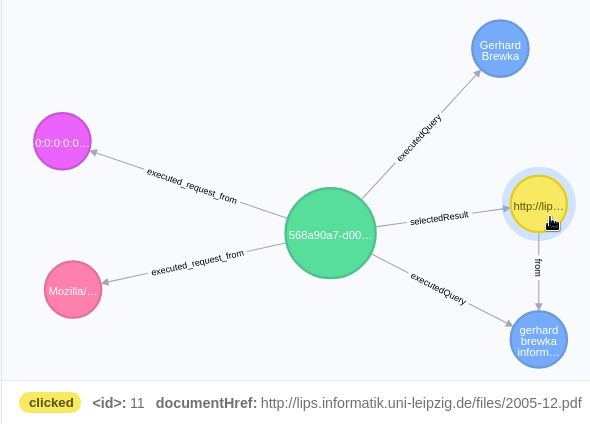
\includegraphics[width=0.99\textwidth]{chapter_query_processing/example_neo4j_visualization.png}
	\caption{Beispielgraph im
	\href{https://neo4j.com/developer/guide-neo4j-browser/}{Neo4j-Browser}
	einer User-Session bestehend aus 2 Anfragen, bei denen bei einer Anfrage ein Ergebniss angeklickt wurde.}
	\label{fig:visualization}
\end{figure}

Die hier vorgestellte Evaluationskomponente funktioniert für alle Clients, welche Cookies erlauben und den \href{}{Referrer-Header}
korrekt setzen.

